\newpage
\section*{Задание 4: Разработка веб-сайта с интерактивными сценариями}
\subsection{Постановка задачи}
Название веб-приложения: Конвертер единиц информации \\
Описание функционала: Поле ввода числового значения и два выпадающих списка для выбора исходной и целевой единицы измерения (биты, байты, КБ, МБ, ГБ, ТБ, ПБ). Переключатель для выбора системы счисления: десятичная (делитель 1000, стандарт SI) или двоичная (делитель 1024, стандарт IEC). По нажатию кнопки «Конвертировать» происходит мгновенный пересчёт с выводом результата.\\
Связь с инженерией данных / ML: Понимание объёмов данных при хранении, передаче и оценке требований к вычислительным ресурсам и инфраструктуре.

\subsection{Гипотеза и системный промпт}
Первая гипотеза: \\
Модель способна самостоятельно спроектировать полное веб-приложение, если чётко описать требования к функционалу, математической логике пересчёта и обработке ошибок. Однако для получения качественного результата необходимо применить технику ролевого моделирования и разделения ответственности (генерировать HTML, CSS и JS последовательно).\\

\indent
Системный промпт для основной модели:
\textit{Ты – Senior Frontend Developer, специализирующийся на создании инженерных калькуляторов и утилит. Твоя задача – помочь разработать одностраничное веб-приложение «Конвертер единиц информации». Пользователь вводит число, выбирает «из» и «в» (биты, байты, КБ, МБ, ГБ, ТБ, ПБ) и переключает режим (SI/1000 или IEC/1024). После нажатия кнопки «Конвертировать» приложение мгновенно вычисляет результат с учётом выбранной базы. Реализуй валидацию ввода: только числа $\ge 0$, поля не должны быть пустыми. При попытке конвертировать одинаковые единицы выводи предупреждение. Интерфейс должен быть современным, адаптивным, с поддержкой тёмной и светлой темы. Отвечай последовательно: сначала предложи структуру HTML, затем CSS, затем JavaScript. После каждого этапа я буду давать обратную связь.}\\

\indent
Обоснование ролевой установки: \\
Роль Senior Frontend Developer направляет модель на использование семантической вёрстки, модульного JS, точной работы с числами (избегание ошибок плавающей запятой) и современных CSS-паттернов, а не примитивных таблиц.

\subsection{Журнал диалога и итераций}
\textbf{Итерация 1 – генерация HTML} \\
\indent
Промпт:
\textit{Сгенерируй чистый HTML-код для приложения конвертера единиц информации. Используй семантические теги (<header>, <main>, <section>, <footer>). Добавь поле ввода для числа (<input type="number">), два выпадающих списка (<select>) для выбора исходной и целевой единицы, переключатель (radio/checkbox) для выбора системы (1000/1024), кнопку «Конвертировать», а также контейнер для вывода результата и блок для сообщений об ошибках. Все интерактивные элементы должны иметь уникальные id. Не добавляй CSS и JS, только структуру.} \\

\indent
Ответ модели:
\lstinputlisting[language=HTML]{z4/index.html}
Анализ результата:
\begin{itemize}
\item Структура логичная, присутствуют все необходимые элементы.
\item Есть контейнер для ошибок, блок вывода результата.
\item Использованы правильные типы инпутов, что упрощает валидацию на стороне браузера.
\end{itemize}

\textbf{Итерация 2 – генерация CSS} \\
\indent
Промпт:
\textit{Теперь сгенерируй CSS для оформления: тёмная тема по умолчанию (фон \#121212, карточка с полями ввода – \#1e1e1e, акцентный синий цвет), адаптивная вёрстка с использованием CSS Grid/Flexbox, стили для кнопки, полей ввода, select. Учти, что на мобильных устройствах элементы должны выстраиваться в одну колонку, а на десктопе – в удобную сетку.} \\

\indent
Ответ модели:
\lstinputlisting{z4/style.css}

\indent
Анализ результата:
\begin{itemize}
\item Дизайн современный, тёмная тема, адаптивность обеспечена через @media.
\item Стили для select и input унифицированы, что улучшает UX.
\end{itemize}

\textbf{Итерация 3 – генерация JavaScript логики} \\
\indent
Промпт:
\textit{
Напиши JavaScript-код, который:
\begin{itemize}
\item По нажатию на кнопку считывает значение, исходную/целевую единицы и систему счисления (1000 или 1024).
\item Проверяет валидность: число $\ge 0$, поля выбраны. При ошибке – выводит сообщение в блок id="error-message".
\item Пересчитывает значение: сначала конвертирует входное значение в базовую единицу (биты), затем из битов – в целевую. Учитывает разницу между битами и байтами (1 байт = 8 бит).
\item Выводит результат с форматированием (до 6 значащих цифр, научная нотация для очень больших/малых чисел).
\item Обрабатывает случай, когда результат уже существует (перезаписывает старый).
\item Используй id элементов: value-input, from-unit, to-unit, base-toggle, convert-btn, result-output, error-message.
\end{itemize}
}

\indent
Ответ модели:
\lstinputlisting{z4/script.js}
Для активации JS надо добавить строчку \texttt{<script src="script.js"></script>} в body в конец. \\

\indent
Анализ результата:
\begin{itemize}
\item Логика пересчёта корректная: используется промежуточная нормализация в биты.
\item Форматирование вывода работает.
\item Но есть потенциальная проблема: при конвертации очень больших чисел JavaScript теряет точность из-за IEEE 754. Добавим обработку через \texttt{Number.toPrecision()} и предупреждение о точности.
\item Также отсутствует очистка ошибки при новом вводе.
\end{itemize}

\textbf{Итерация 4 – улучшение устойчивости (валидация и крайние случаи)} \\
\indent
Промпт:
\textit{Добавь в JavaScript дополнительную защиту:
1. Очистка сообщения об ошибке перед каждым новым нажатием.
2. Если число превышает безопасный предел JS (Number.MAX\_SAFE\_INTEGER), выводи результат в экспоненциальной форме и добавь сноску о возможной погрешности.
3. Запрети конвертацию, если «из» и «в» совпадают.
4. Округляй результат до 4 знаков после запятой для маленьких значений, чтобы не выводить мусорные нули.} \\

\indent
Ответ модели:
\lstinputlisting{z4/script-v2.js}

\indent
Анализ:
Приложение теперь устойчиво к вырожденным случаям, корректно работает с большими числами и даёт понятную обратную связь пользователю.

\subsection{Артефакты}
Итоговый HTML-файл объединяет все три компонента.
Скриншот работающего интерфейса (десктоп):
\begin{figure}[H]
\centering
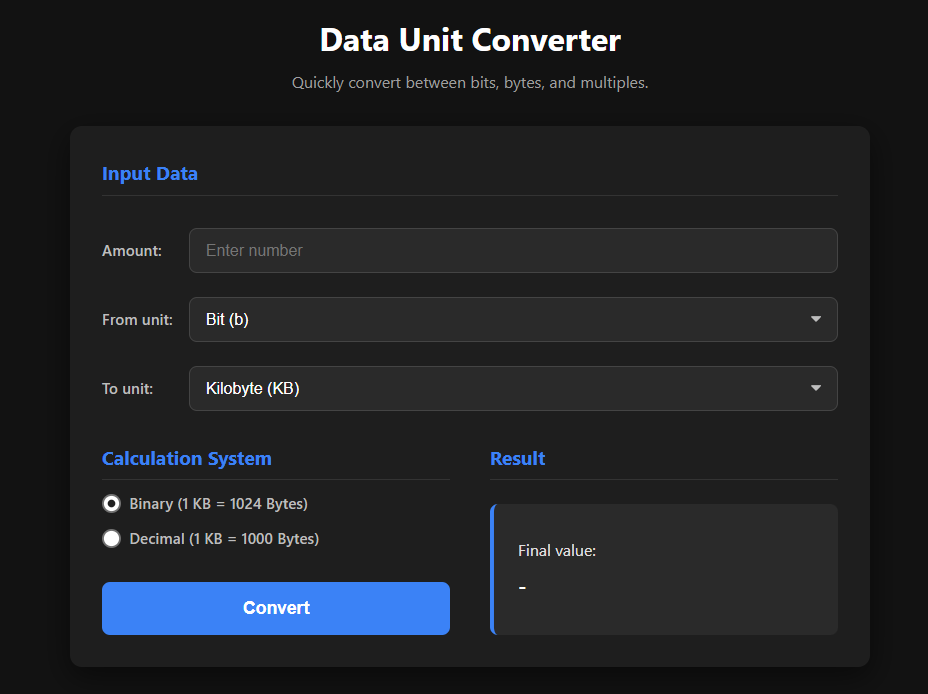
\includegraphics[width=16cm]{z4/s1.png}
\caption{Основной экран конвертера (десктоп)}
\end{figure}

Скриншот результата конвертации с предупреждением о больших числах:
\begin{figure}[H]
\centering
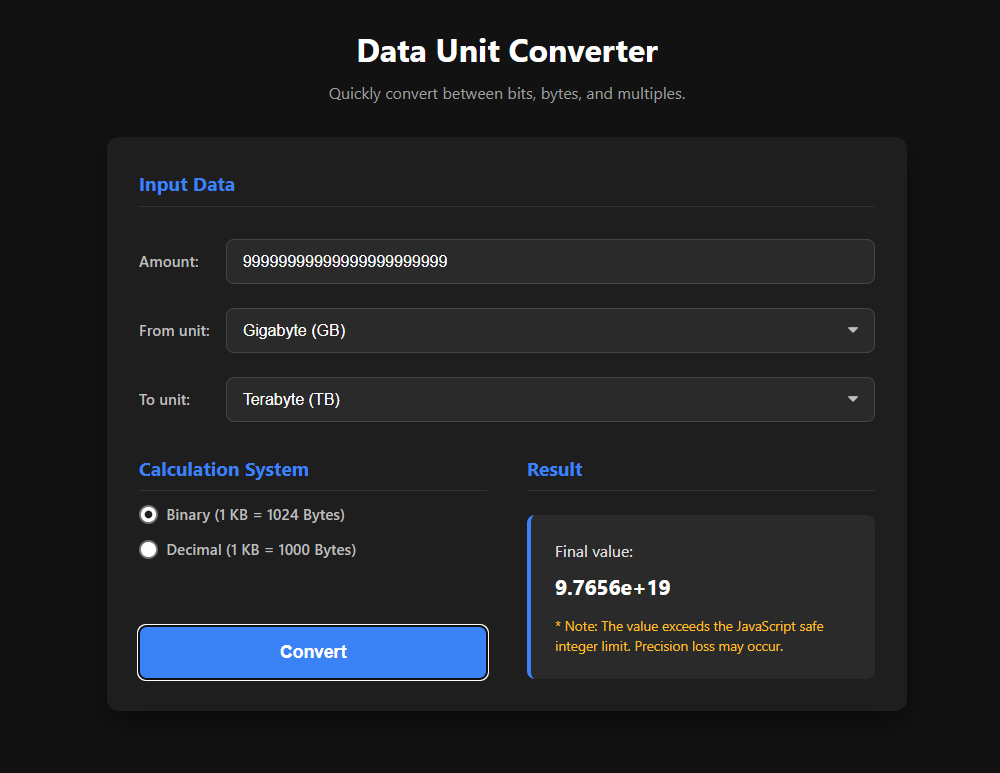
\includegraphics[width=16cm]{z4/s2.png}
\caption{Результат конвертации ГБ в ТБ с экспоненциальной нотацией}
\end{figure}

Скриншот с мобильного устройства:
\begin{figure}[H]
\centering
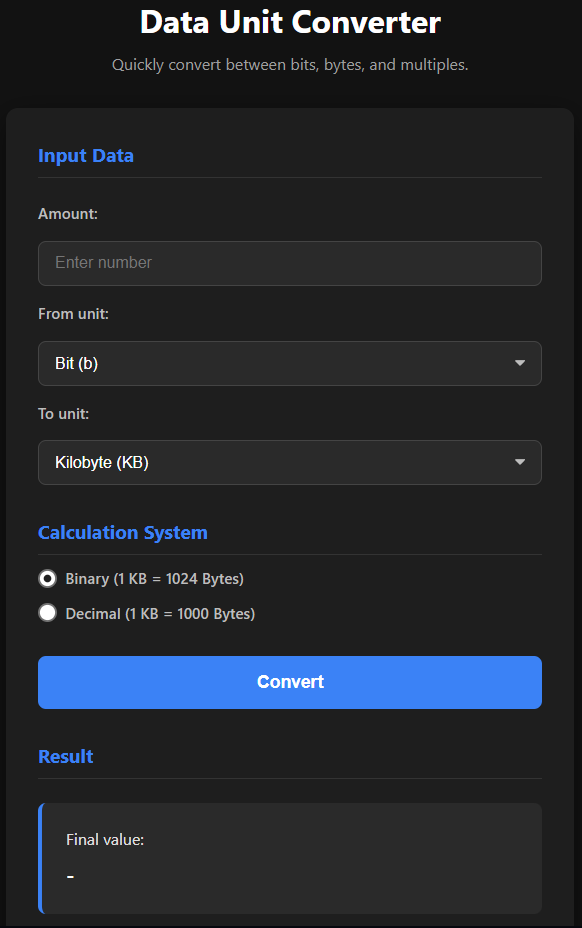
\includegraphics[width=14cm]{z4/s3.png}
\caption{Адаптивный вид на мобильном устройстве}
\end{figure}

\subsection{Сравнение моделей}
Финальный промпт (объединённый, содержащий все требования) был подан контрольной модели без изменений. \\

Результаты сравнения:
\begin{table}[h!]
\centering
\begin{tabular}{|l|p{5cm}|p{5cm}|}
\hline
\textbf{Критерий} & \textbf{модель (a)} & \textbf{модель (b)} \\
\hline
Функциональность & 5 & 5 \\
\hline
Устойчивость  & 5 & 4\\
\hline
Качество кода & 5 & 4 \\
\hline
Галлюцинации & нет & нет \\
\hline
\textbf{Итог} & 5.0 & 4.5\\
\hline
\end{tabular}
\end{table} \\
Итог:
Обе модели справились с задачей хорошо. Основная модель (a) сразу предложила более продуманную логику нормализации через биты и корректно обработала граничные условия с первого раза. Контрольная модель (b) потребовала дополнительной итерации для исправления погрешностей при работе с плавающей запятой, но в целом сгенерировала рабочий код.

\subsection{Вывод}
В ходе выполнения задания наиболее эффективными техниками промпт-инжиниринга оказались:
\begin{itemize}
\item \textbf{Ролевое моделирование} (Senior Frontend Developer) – направляло модель на использование правильных инструментов, семантической вёрстки и модульной архитектуры.
\item \textbf{Разделение ответственности} – последовательная генерация HTML, CSS и JS позволила контролировать качество каждого слоя и легко вносить локальные изменения без поломки всей структуры.
\item \textbf{Итеративное уточнение} – на каждом этапе я анализировал ответ и давал конкретные корректировки (добавить очистку ошибок, обработку больших чисел, запрет одинаковых единиц), что превратило прототип в готовый инструмент.
\end{itemize}
Без этих техник модель могла бы выдать либо упрощённый конвертер без учёта разницы битов/байтов, либо нестабильный код с ошибками точности.
Применение Chain-of-Thought не потребовалось в явном виде, так как задача веб-разработки хорошо структурирована и разбита на слои.\\

\textbf{Приложение А. Итоговый код веб-приложения} \\
\lstinputlisting[language=HTML]{z4/result.html}